\documentclass[12pt, a4paper]{article}
\usepackage{graphicx}
\usepackage{pgfplots}
\usepackage{mathtools}
\usepackage{fancyhdr}
\usepackage{multicol}
\usepackage{cancel}
\usepackage{geometry}
\usepackage{listings}
\usepackage{booktabs}
\usepackage{tabularx}
\usepackage{subfig}
\usepackage{hyperref}
\usepackage{float}
\usepackage{titlesec}
\usepackage{tikz, pgfplots}
\usepackage[utf8]{inputenc}
\usepackage[backend=biber,style=apa]{biblatex}

% Requirement libs
\usetikzlibrary{positioning}

% Options
\nonstopmode % To make sure that you dont have to press input for each error
\geometry{top=1in, left = 1in, right = 1in, bottom=1.2in}
\pgfplotsset{compat=1.18}
\graphicspath{{./figures/}}
\setlength{\columnsep}{0.7cm}

% Metadata
\bibliography{./citations.bib}
\addbibresource{./citations.bib}
\author{Aris Podotas}
\date{today}

% Herlink setup
\hypersetup{
    colorlinks=true,
    linkcolor=blue,
    filecolor=magenta,
    urlcolor=cyan,
    pdftitle={MLICB Assignment 1},
    pdfpagemode=FullScreen,
}

% For the code blocks
\definecolor{codegreen}{rgb}{0.03,0.5,0.03}
\definecolor{codegray}{rgb}{0.5,0.5,0.5}
\definecolor{codepurple}{rgb}{0.58,0,0.82}
\definecolor{backcolour}{rgb}{0.95,0.95,0.95}

% Code block setup
\lstdefinestyle{mystyle}{
    backgroundcolor=\color{backcolour},
    commentstyle=\color{codegreen},
    keywordstyle=\color{magenta},
    numberstyle=\tiny\color{codegray},
    stringstyle=\color{codepurple},
    basicstyle=\ttfamily\footnotesize,
    breakatwhitespace=false,
    breaklines=true,
    captionpos=b,
    keepspaces=true,
    numbers=left,
    numbersep=5pt,
    showspaces=false,
    showstringspaces=false,
    showtabs=false,
    tabsize=4,
    escapeinside = {(*}{*)}
}
\lstset{style=mystyle}

% My custom headers and margins 
\pagestyle{fancy}
\setlength{\headheight}{44pt}
\setlength{\headsep}{18pt}
\lhead{\includegraphics[scale = 0.2]{./figures/bnw unit.png}}
\chead{\quad Data Science and Information Technologies Master’s
National and Kapodistrian University of Athens}
\rhead{}
\lfoot{}
\cfoot{\thepage}
\rfoot{}

% Start
\begin{document}

% Custom title page
\begin{titlepage}
    \centering
    {\huge \textbf{Assignment 2}\par}
    \vspace{0.5cm}
    {\Large \textbf{Name:} Aris Podotas\par}
    \vspace{0.5cm}
    {\large \textbf{University:} National and Kapodistrian University of Athens\par}
    \vspace{0.5cm}
    {\large \textbf{Program:} Data Science and Information Technologies\par}
    \vspace{0.5cm}
    {\large \textbf{Specialization:} Bioinformatics - Biomedical Data\par}
    \vspace{0.5cm}
    {\large \textbf{Lesson:} Machine Learning In Computational Biology\par}
    \vspace{0.5cm}
    {\large \textbf{Date:} May 2025\par}
    \tableofcontents
\end{titlepage}

\begin{multicols}{2}

    \section*{Abstract} \label{sec:abs}

    \section{Introduction} \label{sec:intro}

    \section{Methods} \label{sec:methods}

    \subsection{Implementation} \label{subsec:impl}

    All results were created in the \textit{Python} programming language \cite{noauthor_3132_nodate}. Functionality from \href{https://github.com/ArisPodotas/Assignment-1-MLICB}{this repository} was also used in the analysis.
    \newline

    \subsection{Models} \label{subsec:models}

    Models:
    \newline

    \begin{enumerate} \label{enm:models}
        \item 
        \item 
        \item 
        \item 
        \item 
    \end{enumerate}

    Models were imported from the \textit{sklearn} \cite{noauthor_scikit-learn_nodate} library in \textit{Python} \cite{noauthor_3132_nodate}.
    \newline

    \subsection{Evaluation metrics} \label{subsec:metrics}

    Four evaluation metrics were chosen
    \newline

    \begin{enumerate} \label{enm:metrics}
        \item Root mean squared error
        \item Mean absolute error
        \item R2 score
        \item Median absolute error
    \end{enumerate}

    As a result of knowing about outliers a median metric must be included to compare with the non-median metrics. We will not be using the "Auc" metrics since our task is not fit for it.
    \newline

    \subsection{Confidences} \label{subsec:conf}

    $1000$ iteration \textit{bootstrapping} was done on models for evaluation along with repeated \textit{k-fold cross validation} for $50$ folds, $20$ iterations.
    \newline

    The \textit{sklearn} library \cite{noauthor_scikit-learn_nodate} does not contain a \textit{bootstrapping} function that we can use to call on our models. A protocol was written at \href{https://github.com/ArisPodotas/Assignment-1-MLICB/blob/main/src/functions.py}{our source files}.
    \newline

    Three distinct \textit{bootstrap} implementations were assessed.
    \newline

    \begin{enumerate} \label{enm:bootstrap}
        \item Only altering the training set
        \item Only altering the validation set
        \item Altering both the training and validation set
    \end{enumerate}

    For all models all three were used.
    \newline

    All files can be found at \href{https://github.com/ArisPodotas/Assignment-2-MLICB}{this repository}.
    \newline

    \subsection{Figures} \label{subsec:figs}

    Figures were generated from the \textit{matplotlib} \cite{noauthor_matplotlib_nodate} library, all implementations are available at \href{https://github.com/ArisPodotas/Assignment-1-MLICB/blob/main/src/functions.py}{our source files}.
    \newline

    In all box plots the dotted green line denotes the mean value and the orange line denotes the median.
    \newline

    \subsection{Missing data} \label{subsec:missing}

    Since missing data was found our strategy for the handling of such entries will be to replace the entry with the median value of the feature in questions. We will choose the median to be more resilient to outliers since we will see that the mean has been affected over the median.
    \newline

    \subsection{Classes} \label{subsec:class}

    One class was implemented for the repeated k fold cross validation
    \newline

\end{multicols}

    \begin{figure}[H]
        \begin{center}
            \includegraphics[width=0.95\textwidth]{figures/rcv.png}
        \end{center}
        \caption{Flow chart of cross validation class implementation}\label{fig:class outline}
    \end{figure}

\begin{multicols}{2}

    This figure was made in Excalidraw \cite{}. Only the main aspects of the class are written in the flow diagram since other implementation details are not part of the purpose of the class such as the "__repr__()" magic method.
    \newline

    \subsection{Data transformations} \label{subsec:transforms}

    Most of our data is of continuous variables that need no interpolation of any sort considering there are fields for mean values standard errors and "worst cases". We will convert the diagnosis field to a binary values one where:
    \newline

    \begin{enumerate} \label{enm:casting}
        \item B -> $0$
        \item M -> $1$
    \end{enumerate}

    \subsection{Feature selection} \label{subsec:fselect}

    \subsection{Hyper parameter optimization} \label{subsec:optuna}

    \section{Results} \label{sec:res}

    We are tasked with evaluating this data completely thus we need to identify data types and cast fields to values we can use. Our data was of continuous values variables for all fields but one, that was converted to a binary field.
    \newline

    \subsection{Data Exploration} \label{subsec:expl}

\end{multicols}

    \begin{figure}[H]
        \begin{center}
            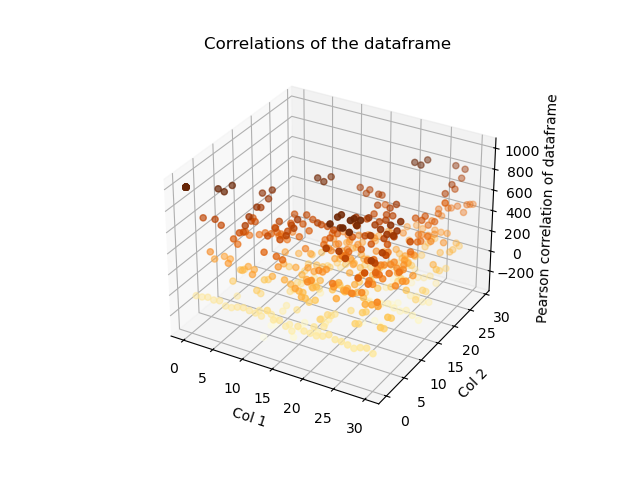
\includegraphics[width=0.95\textwidth]{figures/Correlations of the dataframe.png}
        \end{center}
        \caption{Pearson correlation of all feature pairs}\label{fig:corr}
    \end{figure}

\begin{multicols}{2}

    We can see that there is a lot of pruning to be done for features that are correlated in Figure~\ref{fig:corr}.
    \newline

\end{multicols}

    \begin{figure}[H]
        \begin{center}
            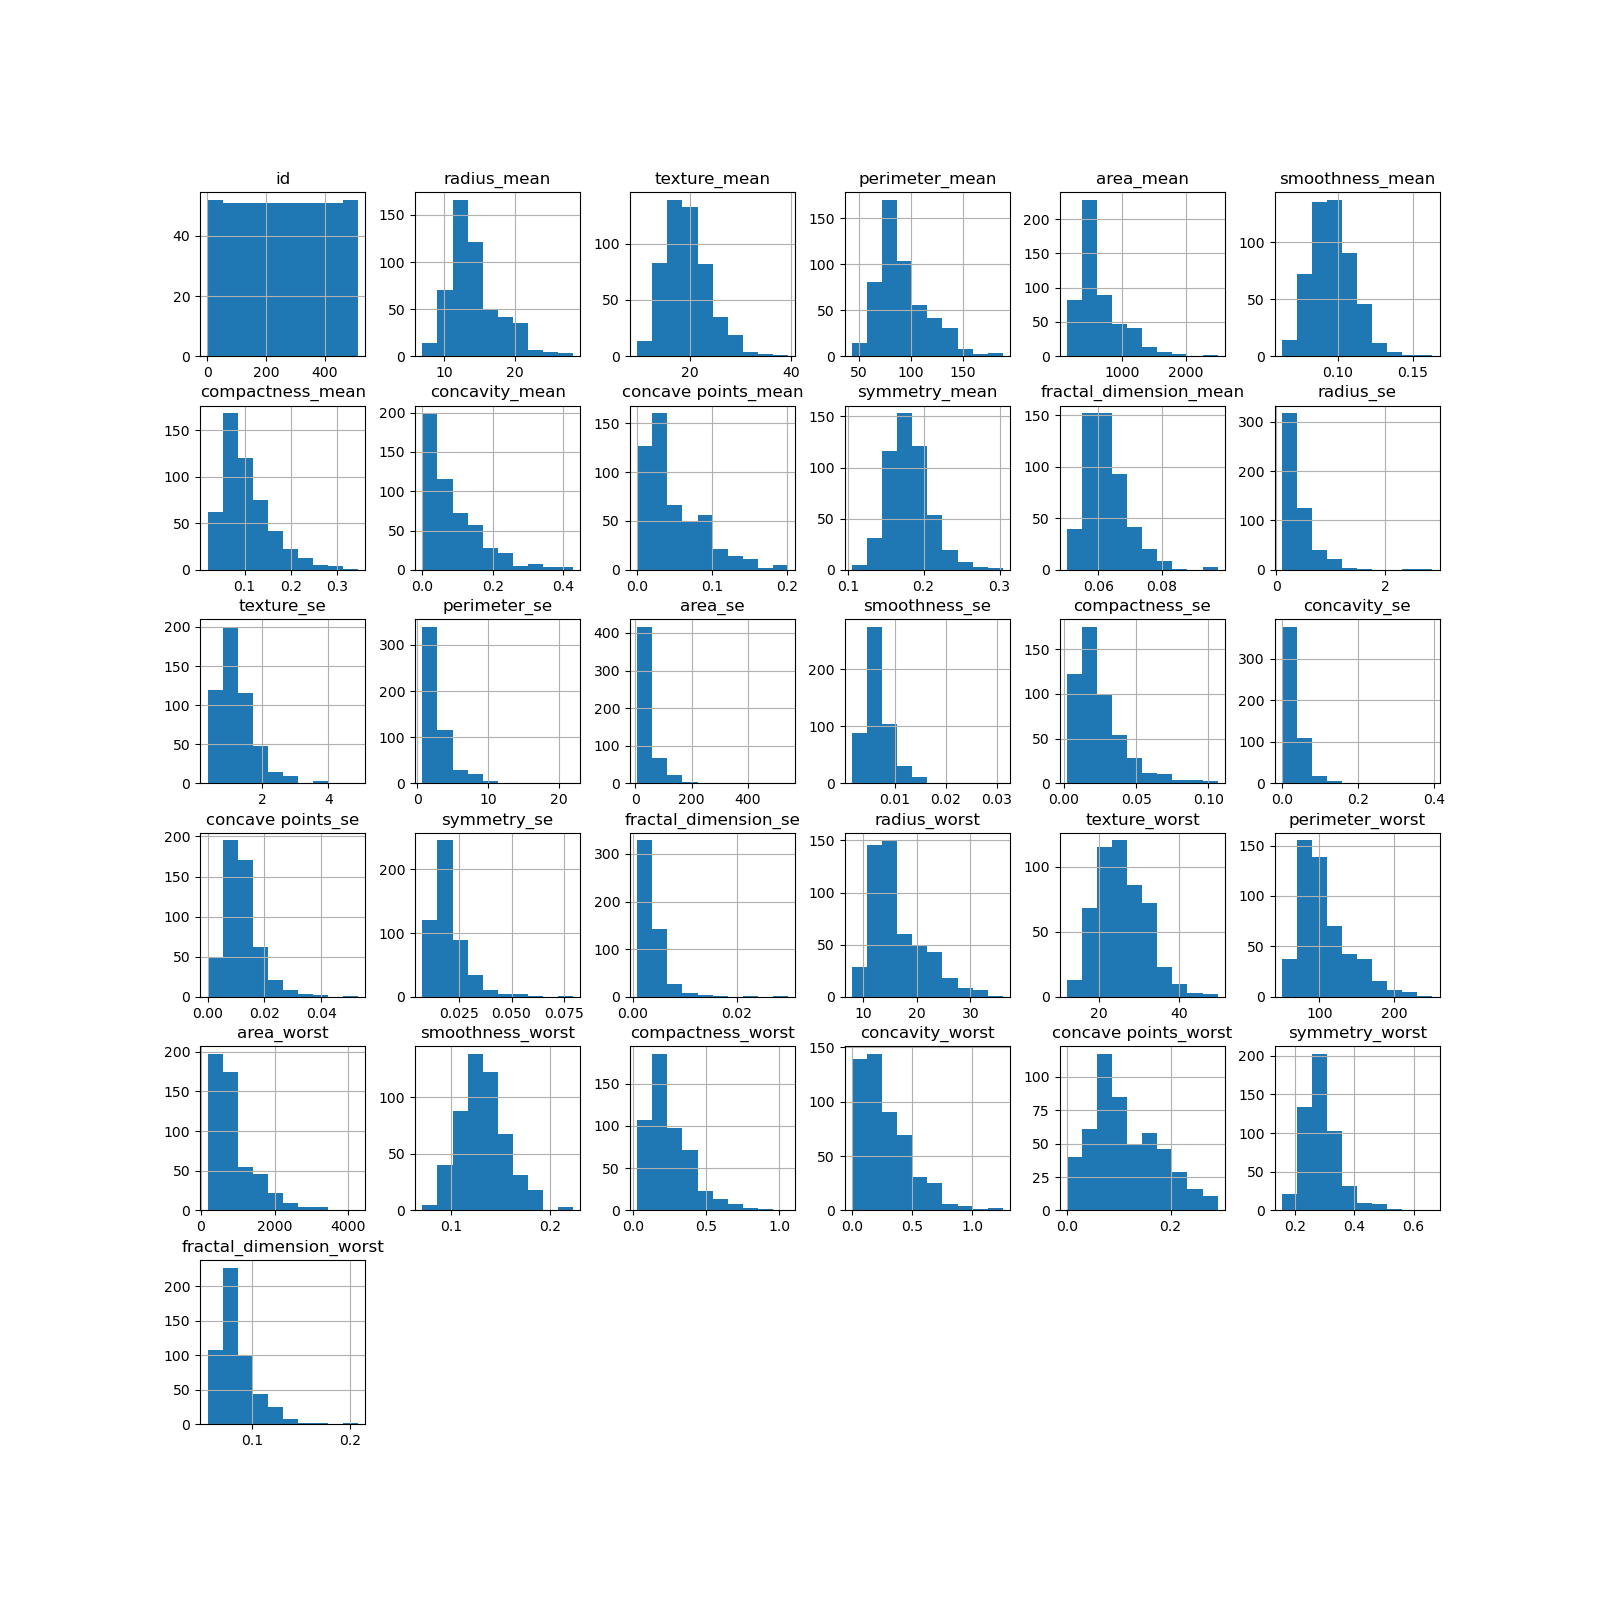
\includegraphics[width=0.95\textwidth]{figures/Data feature histograms.png}
        \end{center}
        \caption{Distribution of values for each feature}\label{fig:hists}
    \end{figure}

\begin{multicols}{2}

    We can make some sort of comment on the appearance of the central limit theorem in Figure~\ref{fig:hists} considering we get a Gaussian looking distribution \cite{} from taking the mean values of feature's distributions.
    \newline

    Descriptive statistics were calculated for the initial data in the \href{}{respective notebook} and then saved to \href{}{this comma separated values file}
    \newline

    \subsection{Baseline} \label{subsec:baseline}

    \subsection{Feature selection} \label{subsec:fs}

    \section{Conclusions} \label{sec:conc}

    \section{Disclaimer} \label{sec:disc}

    Large language models (LLM's) were used during the assignment.

    \subsection{LLM} \label{subsec:llms}

    Open AI: Chat GPT 4.0 \cite{noauthor_chatgpt_nodate}

    \subsection{Purpose} \label{subsec:llmUse}

    \begin{enumerate} \label{enm:llm}
        \item To ask if concepts already exist in some dependency.
        \item For acquisition of the relative documentation.
        \item For helping with the \LaTeX table formatting in this report for time efficiency.
        \item Debugging help
    \end{enumerate}

    \section{Citations} \label{sec:citations}

    \printbibliography

\end{multicols}

\end{document}

